% Sección C · Modelo dimensional y una sola definición (componente C, 10 %). Reemplaza al «Modelo dimensional» de la E1.
% Requiere en el preámbulo: graphicx, booktabs, array. Las cifras salen de E2/output/cifras.md.

\section{Modelo dimensional y una sola definición}
\label{sec:modelo}

Modelamos un solo proceso de negocio, la venta: cada vez que se factura una línea de vino. Es una tabla de hechos transaccional con cuatro dimensiones a un salto (figura~\ref{fig:modelo}); la fuente viene normalizada en tablas encadenadas (ventas, mercados, zonas) y la aplanamos en una estrella porque país y zona son niveles de una misma jerarquía.

\begin{quote}
\textbf{Grano.} Una fila de \texttt{fact\_venta} es una línea de venta facturada: un producto de una añada, vendido a un cliente en una fecha.
\end{quote}

\begin{figure}[!htbp]
  \centering
  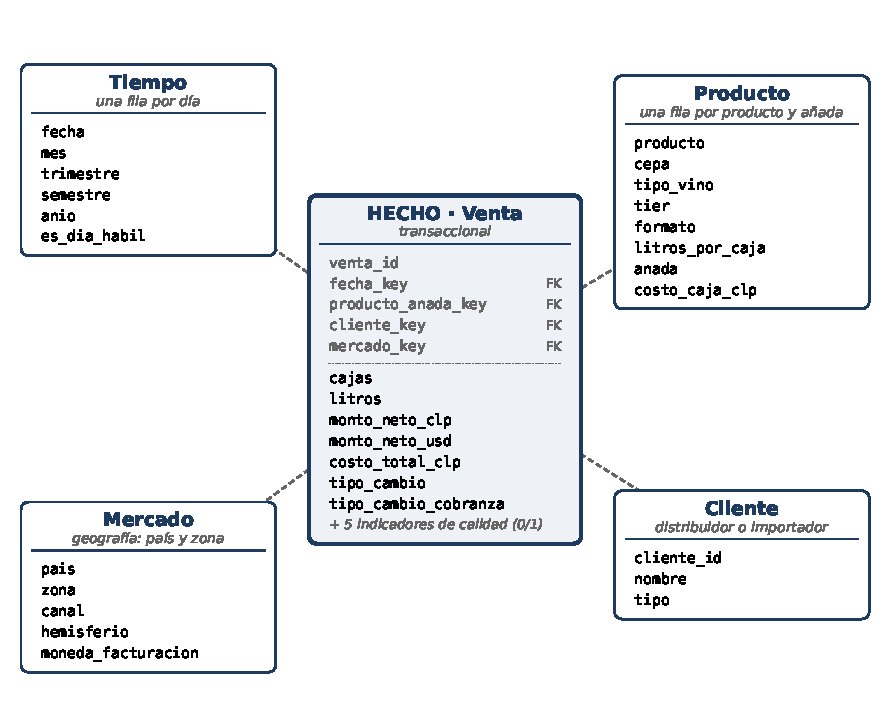
\includegraphics[width=0.47\textwidth]{modelo_estrella.pdf}
  \caption{Modelo estrella de la venta. Diccionario de datos, con la unidad de cada campo, en el anexo~C. Fuente: elaboración propia.}
  \label{fig:modelo}
\end{figure}

\paragraph{Por qué este grano.} No hay en la fuente un nivel más fino, y uno más grueso destruye la pregunta: para separar precio de mezcla, cada fila debe conservar su tier y sus litros. Por lo mismo, el hecho guarda solo lo que se suma (cajas, litros, montos en pesos y en dólares, costo) y nunca el precio por litro: una razón de sumas no es aditiva y se calcula en cada corte. De las 13.845 filas, 10.672 son exportaciones facturadas en 2025 y forman el universo de la métrica.

\paragraph{Las dimensiones.} \texttt{dim\_producto} tiene una fila por producto y añada (96), porque el costo por caja depende de la añada; ahí viven el tier y \texttt{litros\_por\_caja}. \texttt{dim\_mercado} trae el canal y el hemisferio, que fija los días de cobranza, y \texttt{dim\_tiempo} el semestre y si el día tuvo dólar publicado. Quedan fuera el embarque, otro proceso con su propio grano que solo corrige las cajas cargadas en botellas, el vendedor, redundante con la zona, y el flete y los aranceles, que no están en ninguna fuente.

\paragraph{Qué cambió respecto de la E1, y por qué.} El grano y las dimensiones no cambiaron: ninguna observación los cuestionó, y la de la P1 pedía explicarlos con más detención, no rehacerlos. Al hecho se le agregaron cinco columnas para que cada escenario de la sección~\ref{sec:metrica} salga de la misma tabla y no de una segunda cadena: el dólar a la fecha estimada de cobranza y a la de embarque, la marca de costo imputado, y las cajas y el monto tal como venían en el ERP. Con las marcas que ya tenía (monto recalculado, cajas corregidas, moneda imputada), la métrica se puede recalcular con cualquier corrección apagada.

\paragraph{La métrica, definida una sola vez.} Las fórmulas viven en un solo objeto del oro: la \emph{metric view} \texttt{oro.mv\_vallehondo} de Unity Catalog, que es la capa semántica de la cadena (tabla~\ref{tab:medidas}). Lee de \texttt{agg\_escenarios}, que guarda solo sumas de \texttt{fact\_venta} por semestre, mes, mercado, tier y formato para cada uno de los 60 escenarios (4 monedas y fechas del dólar, 3 equivalencias de litros por caja y 5 combinaciones de correcciones); las razones se calculan al consultar.

\begin{table}[!htbp]
\centering\small
\caption{Medidas de la definición única (\texttt{oro.mv\_vallehondo}).}
\label{tab:medidas}
\begin{tabular}{@{}l l l@{}}
\toprule
\textbf{Medida} & \textbf{Fórmula} & \textbf{Unidad} \\
\midrule
\texttt{precio\_por\_litro} & $\sum$ ingreso neto $\div$ $\sum$ litros & USD/L o CLP/L \\
\texttt{margen\_por\_litro} & $\sum$ (ingreso neto $-$ costo de producto) $\div$ $\sum$ litros & CLP/L \\
\texttt{participacion\_gran\_reserva} & litros de gran reserva $\div$ litros & \% \\
\texttt{cobertura\_costo\_real} & litros con costo no imputado $\div$ litros & \% \\
\bottomrule
\end{tabular}
\end{table}

\noindent El tablero, las vistas de la descomposición y el paso que escribe las cifras del informe consultan estas medidas; no hay una segunda fórmula en Python ni en el tablero. Por eso el precio medio por litro tiene el mismo nombre y el mismo número en el informe, en \texttt{cifras.md} y en la pantalla: 4,574 y 5,085 USD/L, +11,2\,\%. Las definiciones alternativas de la E1, los litros por caja de 18 o 4,5 y la conversión a pesos con otra fecha, siguen disponibles como filtros del prototipo: la contraparte las ve sin que recalculemos nada.
